\section{软件设计}
\label{sec:introduction}

\begin{frame}
  \begin{center}
    \Huge{\textcolor{red}{软件设计}}
  \end{center}
\end{frame}

\subsection{简单设计}

\begin{frame}{为什么要做软件设计?}
  \begin{figure}
    \centering
    
\includegraphics[width=0.5\textwidth]{why.png}
  \end{figure}
\end{frame}

\begin{frame}{拥抱变化}
  \begin{figure}
    \centering
    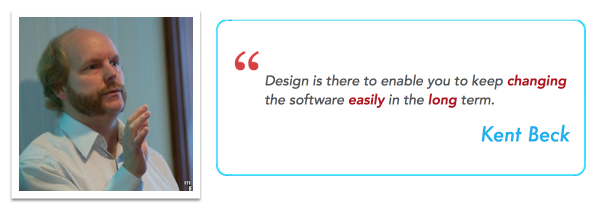
\includegraphics[width=1.0\textwidth]{why-design.png}
  \end{figure}
\end{frame}

\begin{frame}
  \begin{center}
    \huge{\textcolor{red}{什么是好的软件设计?}}
  \end{center}
\end{frame}

\begin{frame}{设计初衷}
  \begin{figure}
    \centering
    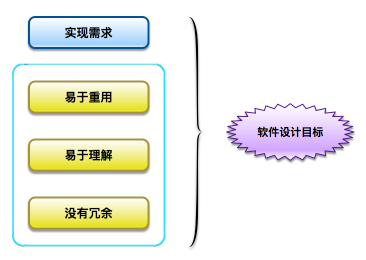
\includegraphics[width=0.7\textwidth]{design-goal.png}
  \end{figure}
\end{frame}

\begin{frame}{易于重用}
  \begin{figure}
    \centering
    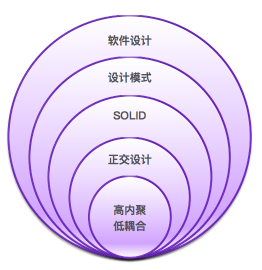
\includegraphics[width=0.5\textwidth]{methodology.png}
  \end{figure}
\end{frame}

\begin{frame}{易于理解}
  \begin{columns} 
  \begin{column}{0.3\textwidth}
  \begin{enumerate}
    \item \alert{Clean Code}
    \item \alert{Idioms}
    \item \alert{Patterns}
  \end{enumerate}
  \end{column}  

  \begin{column}{0.7\textwidth}
  \begin{figure}
    \centering
    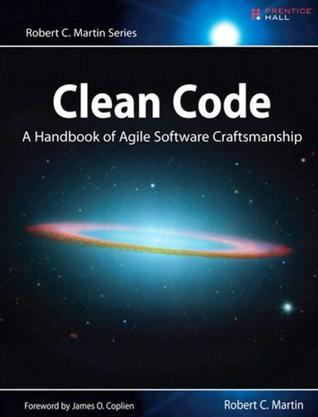
\includegraphics[width=0.5\textwidth]{clean-code.jpg}
  \end{figure}
  \end{column}
  \end{columns}   
\end{frame}

\begin{frame}{没有冗余}
  \begin{enumerate}
    \item \alert{YAGNI}: You Ain't Gonna Need It
    \item \alert{KISS}: Keep it Simple, Stupid
  \end{enumerate}
\end{frame}

\begin{frame}{简单设计}
  \begin{block}{以下4个原则的重要程度依次降低}
    \begin{enumerate}
    \item \alert{通过测试}:完成功能
    \item \alert{没有重复}:易于重用
    \item \alert{意图明确}:易于理解
    \item \alert{没有冗余}:恰如其分
    \end{enumerate}
  \end{block}
\end{frame}

\begin{frame}
  \begin{center}
    \huge{\textcolor{red}{如何重用软件?}}
  \end{center}
\end{frame}

% \begin{frame}{模块化设计}
% \begin{enumerate}
%   \item \alert{一个出发点}:模块化设计
%   \item \alert{两个问题}:分解与组合(高内聚,低耦合)
%   \item \alert{三方关系}:客户,实现,API
%   \item \alert{四个策略}:正交设计原则  
% \end{enumerate}
% \end{frame}

\begin{frame}{一个出发点:模块化设计}
  \begin{figure}
    \centering
    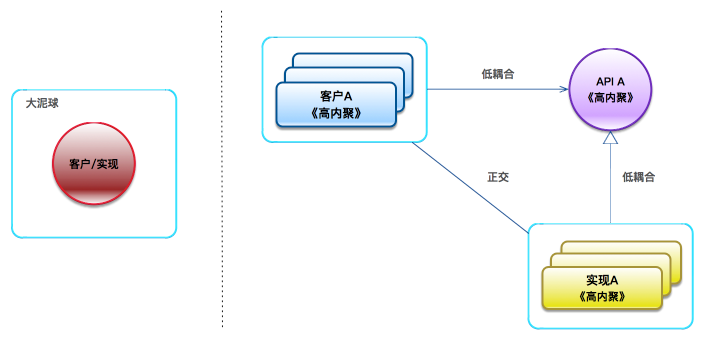
\includegraphics[width=1.0\textwidth]{module-design.png}
  \end{figure}
\end{frame}

\begin{frame}{两个基本问题:分解与组合}
\begin{enumerate}
  \item \alert{分解:} 当我们划分模块时,要让每个模块都尽可能高内聚
  \item \alert{组合:} 当定义模块之间的API时,需要让双方尽可能低耦合 
\end{enumerate}
\end{frame}

\begin{frame}{人类认知}
  \begin{figure}
    \centering
    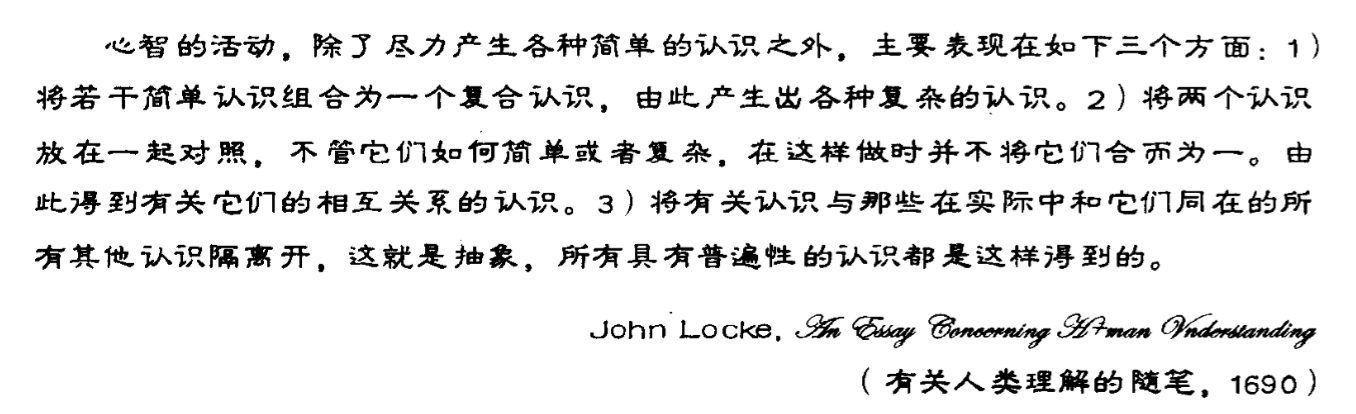
\includegraphics[width=1.0\textwidth]{cognition.png}
  \end{figure}
\end{frame}

\begin{frame}{高内聚:Do One Thing, Do It Well}
\begin{enumerate}
  \item \alert{紧密关联的事物应该放在一起。}
  \item \alert{只有关联紧密的事物才应该被放到一起。}  
\end{enumerate}
\end{frame}

\begin{frame}{职责的定义:变化的原因}
\begin{enumerate}
  \item \alert{SRP:} 一个模块有且仅有一个发生变化的原因
  \item \alert{变化原因:} 一个变化会导致整个模块内包含的各个元素都要发生变化,那么就不能分离它们;否则,将引入不必要的复杂度。
  \item \alert{变化驱动:} 当且仅当变化发生时,分离变化的轴线才有意义。
\end{enumerate}
\end{frame}

\begin{frame}[fragile]{习惯思维:以概念的方式识别职责}
  \begin{java}
public interface Modem {
  void dial(String pno);
  void hangup();
  void send(char c);
  char recv(); 
}
  \end{java}
\end{frame}

\begin{frame}[fragile]{分离职责}
  \begin{java}
public interface Connection {
  void dial(String pno);
  void hangup();
}

public interface DataChannel {
  void send(char c);
  char recv(); 
}
  \end{java}
\end{frame}

\begin{frame}[fragile]{面向对象:小类,大对象}
\begin{enumerate}
  \item \alert{类:} 模块化设计的手段;
  \item \alert{对象:} 映射真正的领域模型。
\end{enumerate}
\end{frame}

\begin{frame}{低耦合}
\begin{enumerate}
  \item \alert{耦合性:} 强调模块之间的关联紧密程度
  \item \alert{低耦合:} 模块之间尽可能地互不影响
\end{enumerate}
\end{frame}

\begin{frame}{API设计}
\begin{enumerate}
  \item \alert{最少知识}:应该让客户尽可能地知道最少的知识
  \item \alert{最小依赖}:不应该强迫客户依赖它不需要的东西
  \item \alert{依赖于抽象,而不是实现}:站在需求的角度,而不是实现方式的角度定义API    
\end{enumerate}
\end{frame}

\begin{frame}{四个策略:正交设计}
  \begin{figure}
    \centering
    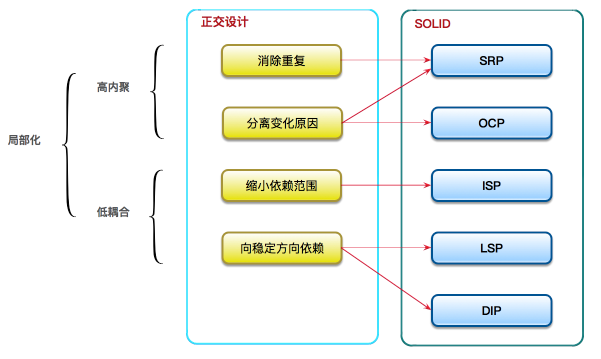
\includegraphics[width=0.95\textwidth]{orthogonal-design.png}
  \end{figure}
\end{frame}

\begin{frame}{拥抱变化}
  \begin{block}{应对变化} 
    \begin{enumerate}
    \item \alert{一个变化导致多处散弹修改}:消除重复
    \item \alert{多个变化导致一处频繁修改}:分离变化
    \end{enumerate}
  \end{block}

  \begin{block}{变化发生时,消除不必要的修改} 
    \begin{enumerate}
    \item \alert{不依赖不必要的依赖}:缩小依赖范围
    \item \alert{不依赖不稳定的依赖}:向着稳定的方向依赖
    \end{enumerate}
  \end{block}
\end{frame}

\subsection{消除重复}

\begin{frame}[fragile]{重复:万恶之源}
  \begin{enumerate}
    \item \alert{完全重复}
    \item \alert{参数型重复}
    \item \alert{功能型重复}    
    \item \alert{结构型重复}              
    \item \alert{调用型重复}
    \item \alert{回调型重复}            
  \end{enumerate}
\end{frame}

\begin{frame}[fragile]{完全重复}
  \begin{figure}
    \centering
    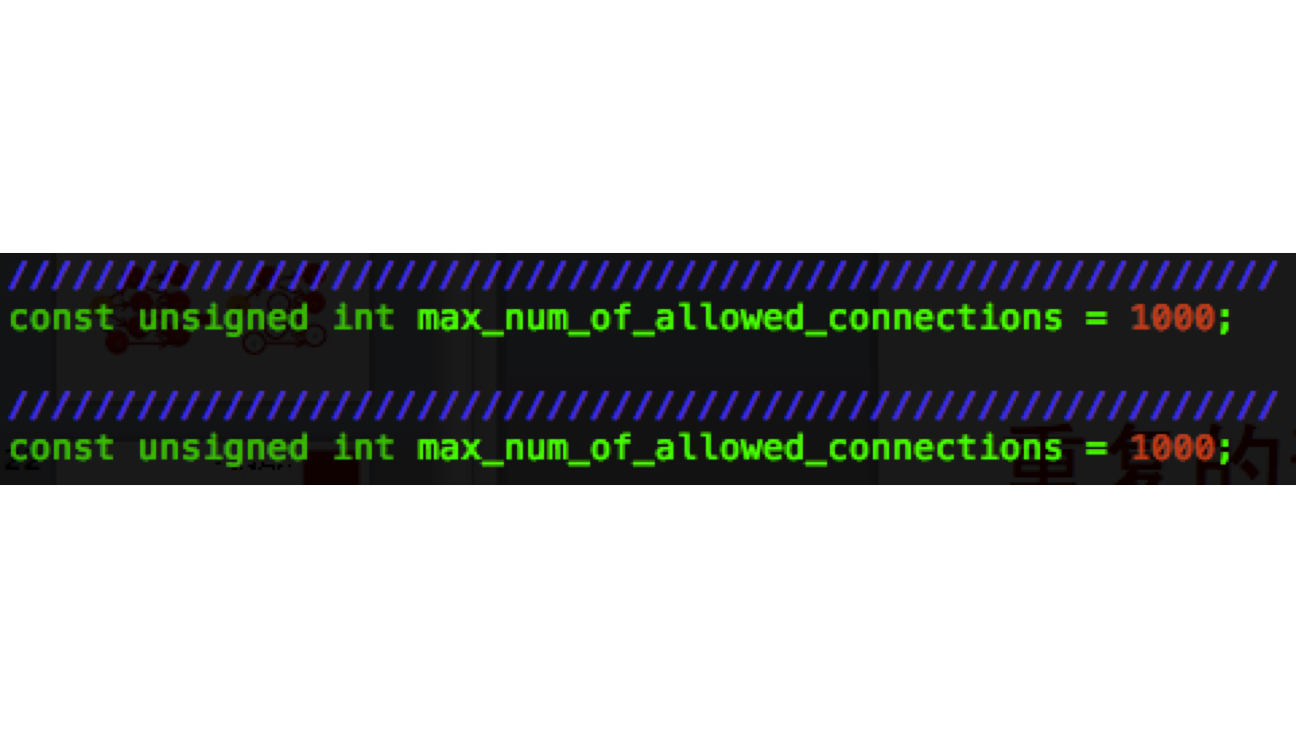
\includegraphics[width=0.95\textwidth]{full-duplication.png}
  \end{figure}
\end{frame}


\begin{frame}[fragile]{参数型重复}
  \begin{figure}
    \centering
    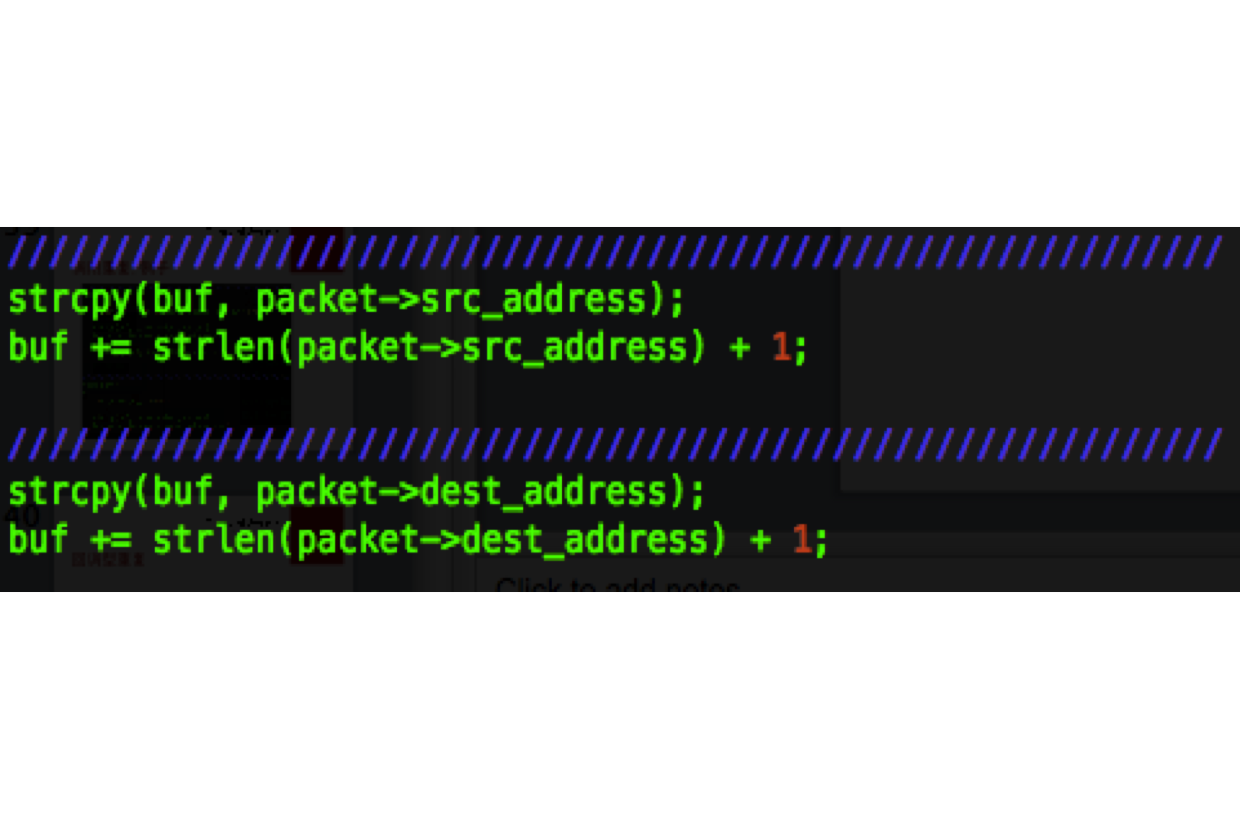
\includegraphics[width=0.95\textwidth]{parameter-duplication.png}
  \end{figure}
\end{frame}

\begin{frame}[fragile]{功能型重复}
  \begin{figure}
    \centering
    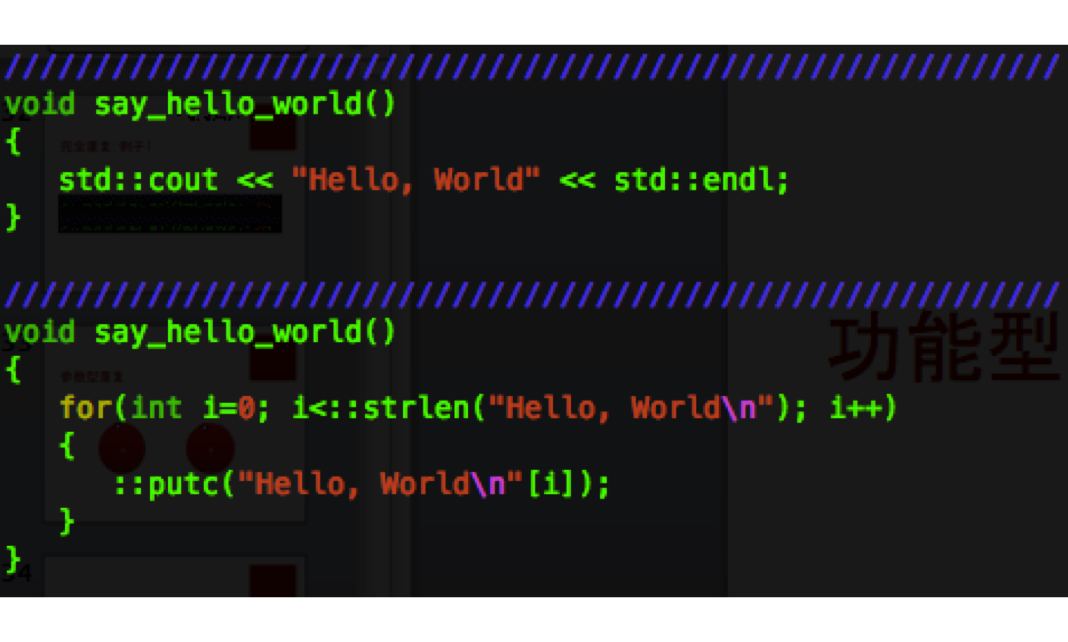
\includegraphics[width=0.95\textwidth]{function-duplication.png}
  \end{figure}
\end{frame}

\begin{frame}[fragile]{结构型重复}
  \begin{figure}
    \centering
    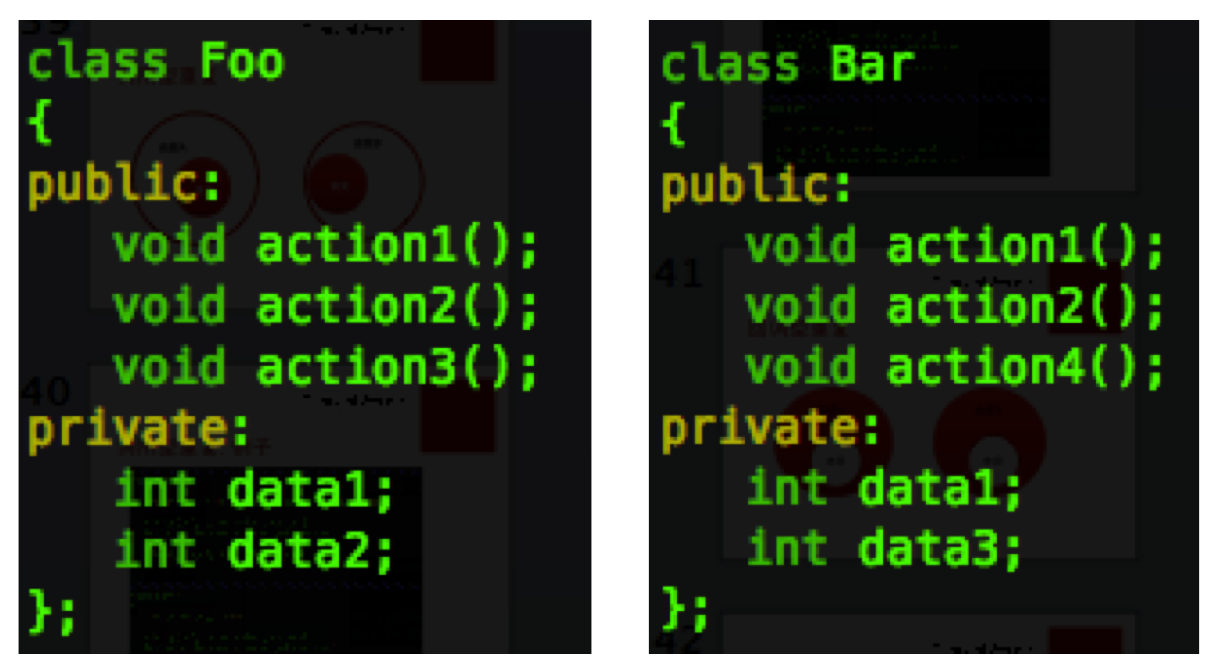
\includegraphics[width=0.7\textwidth]{struct-duplication.png}
  \end{figure}
\end{frame}

\begin{frame}[fragile]{调用型重复}
  \begin{figure}
    \centering
    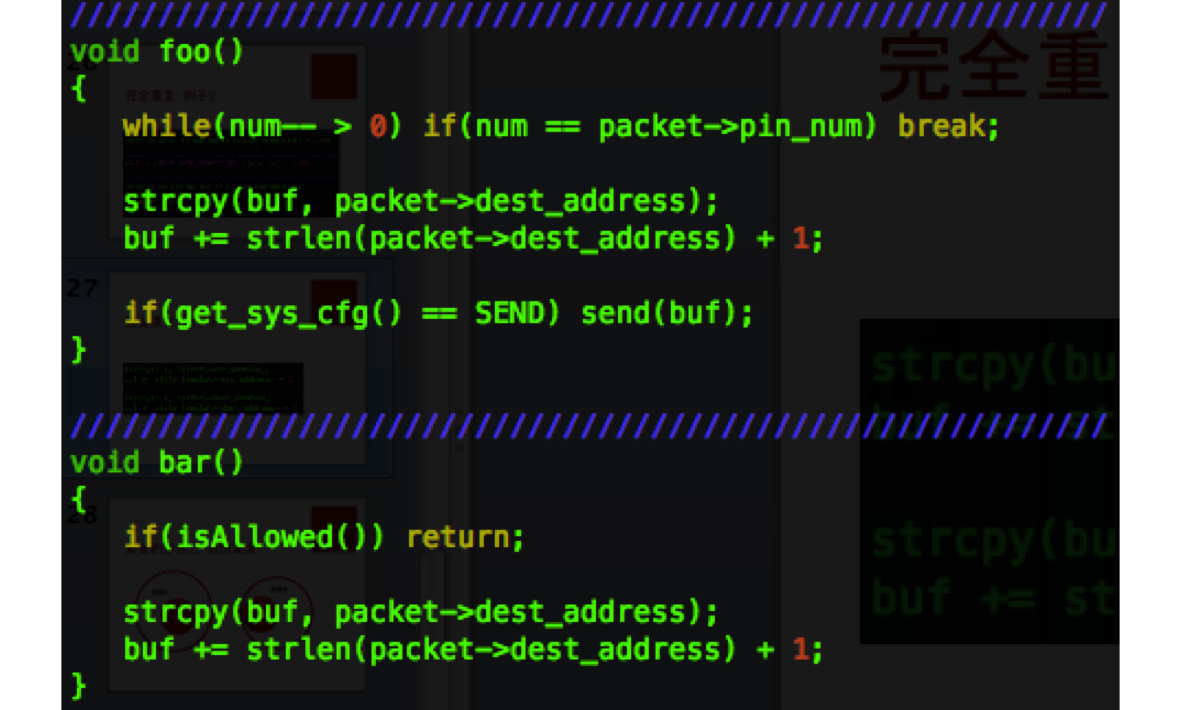
\includegraphics[width=0.95\textwidth]{invoke-duplication.png}
  \end{figure}
\end{frame}

\begin{frame}[fragile]{回调型重复}
  \begin{figure}
    \centering
    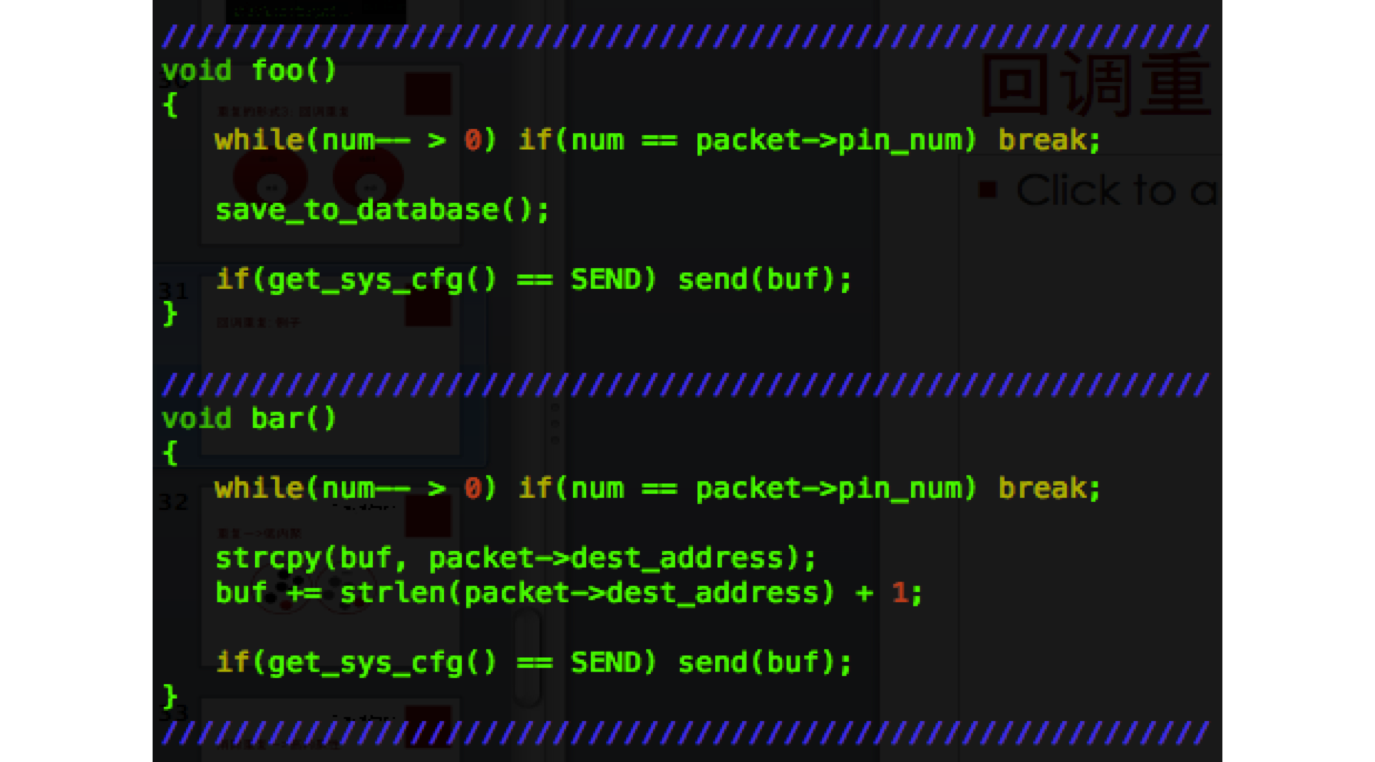
\includegraphics[width=0.95\textwidth]{callback-duplication.png}
  \end{figure}
\end{frame}

\begin{frame}[fragile]{重复: 低内聚}
  \begin{figure}
    \centering
    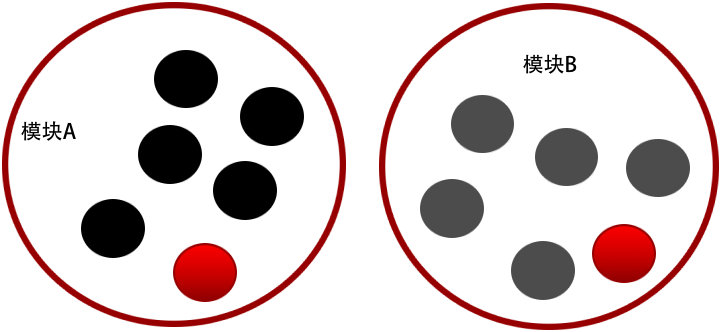
\includegraphics[width=0.6\textwidth]{duplication-low-cohesion.png}
  \end{figure}
\end{frame}

\begin{frame}[fragile]{重复: 高耦合}
  \begin{figure}
    \centering
    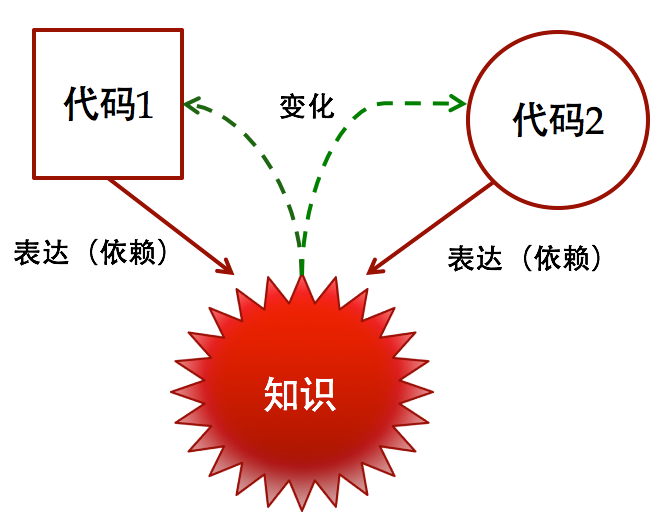
\includegraphics[width=0.6\textwidth]{duplication-def.png}
  \end{figure}
\end{frame}

\begin{frame}[fragile]{消除重复: 高内聚,低耦合}
  \begin{figure}
    \centering
    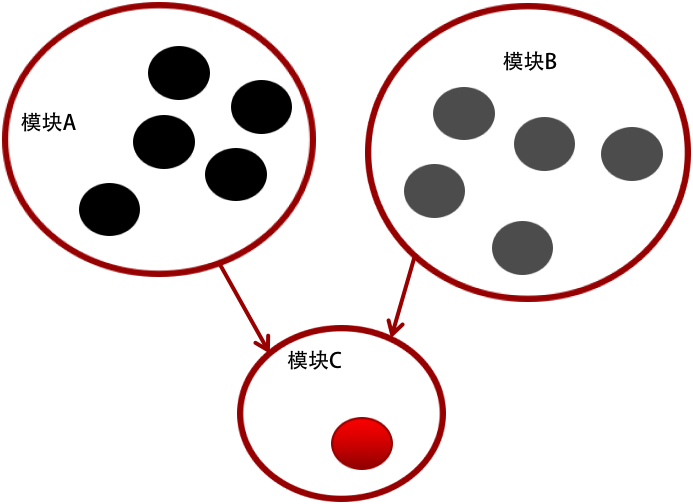
\includegraphics[width=0.6\textwidth]{dry-hign-cohesion.png}
  \end{figure}
\end{frame}

\begin{frame}[fragile]{消除重复: SRP}
  \begin{figure}
    \centering
    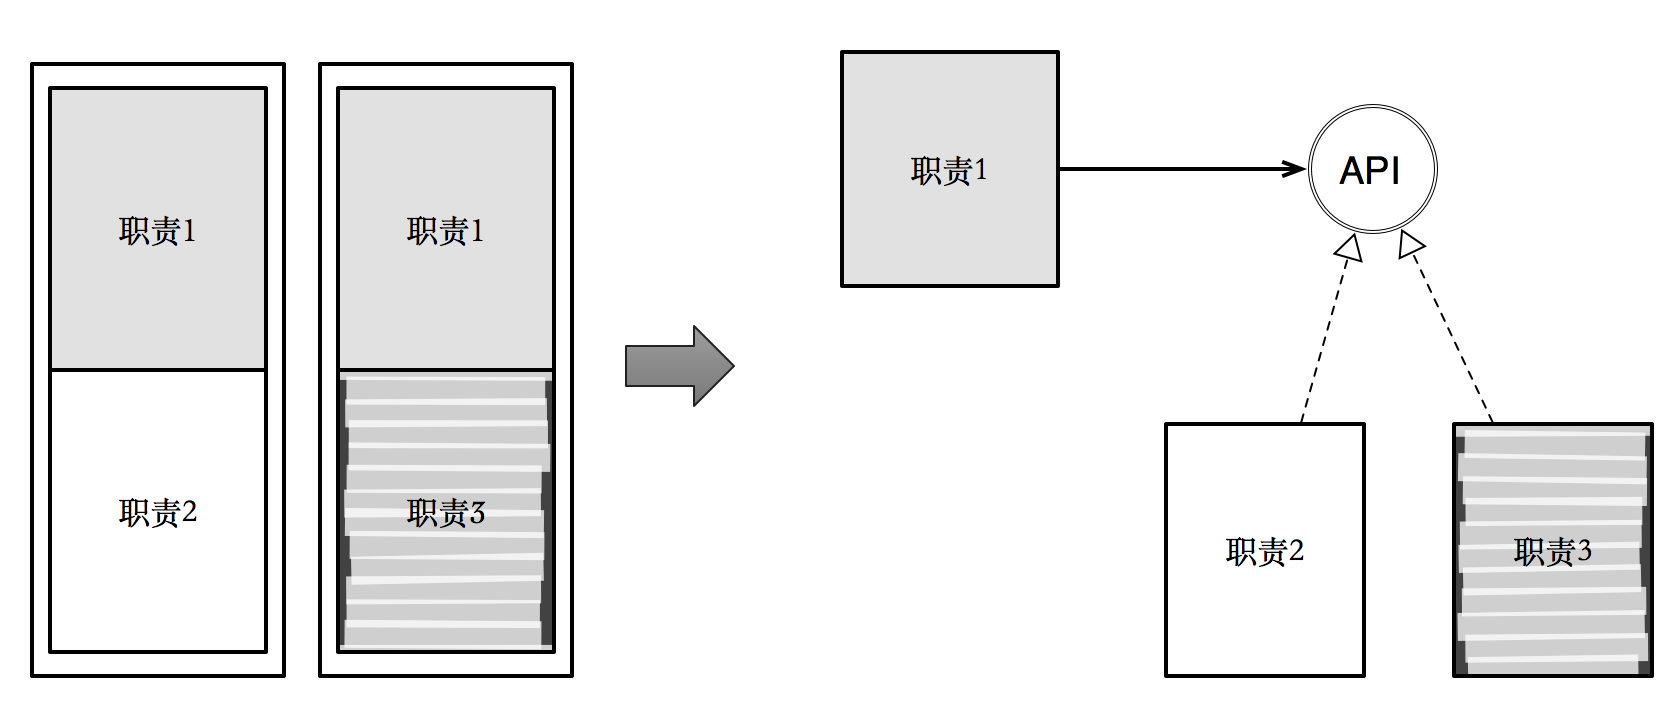
\includegraphics[width=0.95\textwidth]{srp1.png}
  \end{figure}
\end{frame}

\subsection{分离关注点}

\begin{frame}[fragile]{排序:从高到低}
  \begin{figure}
    \centering
    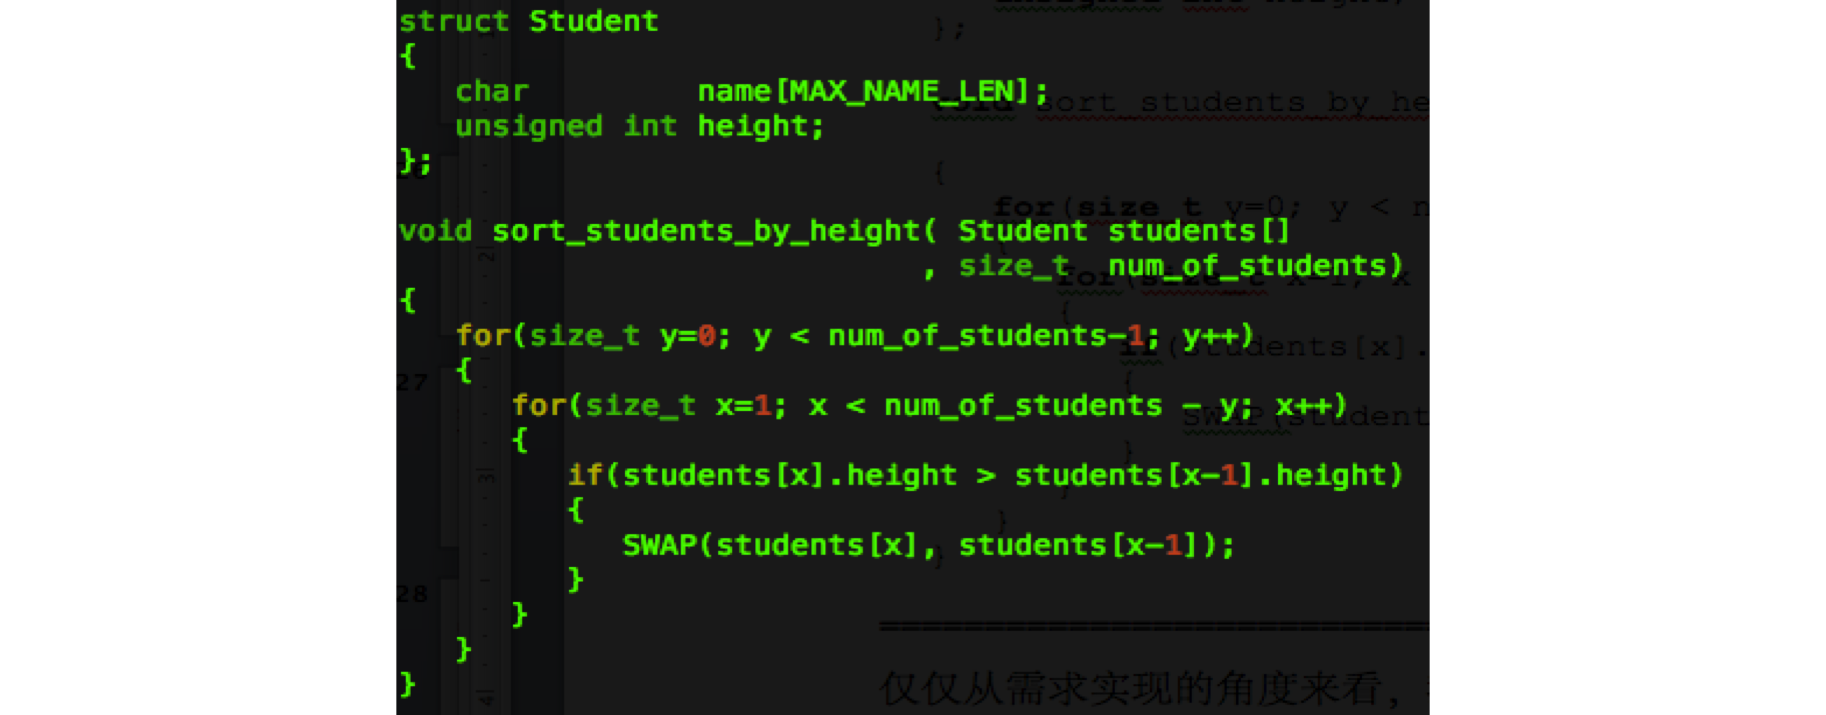
\includegraphics[width=1.2\textwidth]{sort.png}
  \end{figure}
\end{frame}

\begin{frame}[fragile]{变化原因}
  \begin{enumerate}
    \item \alert{排序算法}
    \item \alert{排序对象}
    \item \alert{比较准则}            
  \end{enumerate}
\end{frame}

\begin{frame}[fragile]{分离关注点}
  \begin{figure}
    \centering
    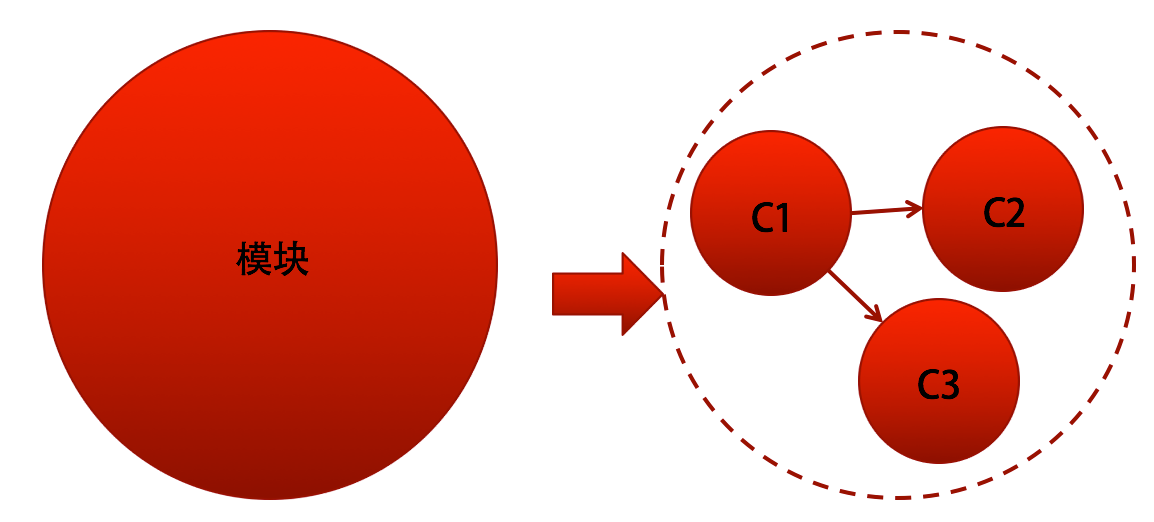
\includegraphics[width=0.7\textwidth]{soc.png}
  \end{figure}
\end{frame}

\begin{frame}[fragile]{分离关注点: SRP}
  \begin{figure}
    \centering
    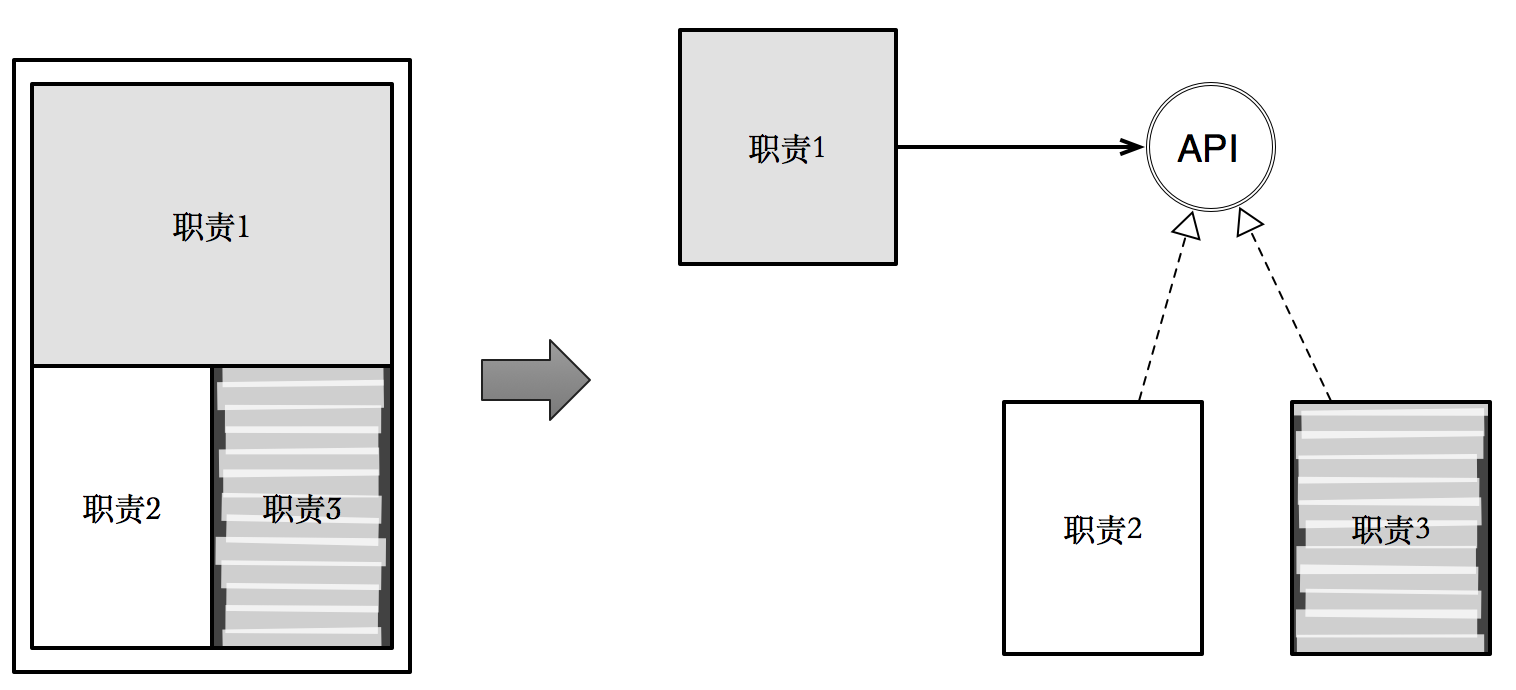
\includegraphics[width=0.95\textwidth]{srp2.png}
  \end{figure}
\end{frame}

\begin{frame}[fragile]{分离关注点: OCP}
  \begin{figure}
    \centering
    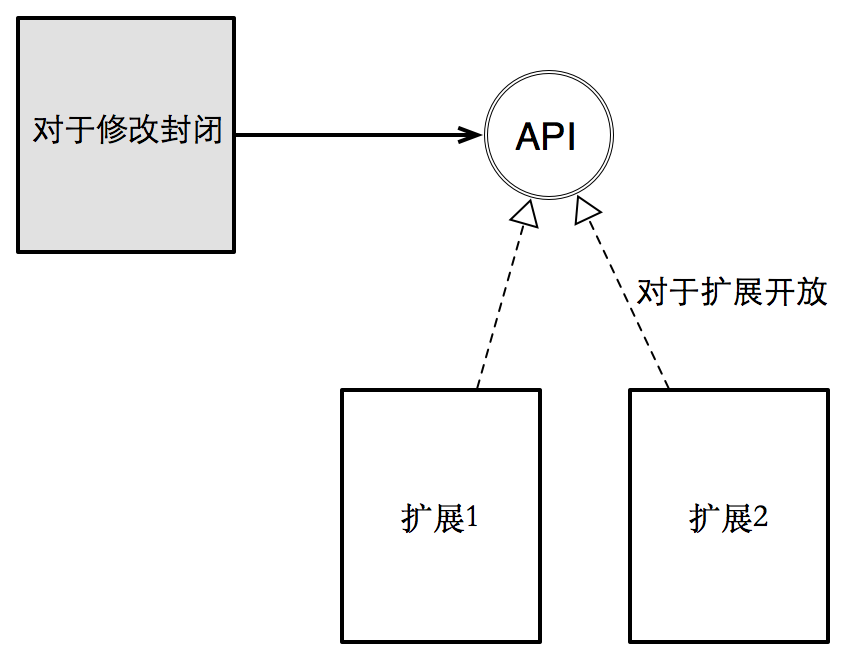
\includegraphics[width=0.7\textwidth]{ocp.png}
  \end{figure}
\end{frame}

\subsection{缩小依赖范围}

\begin{frame}[fragile]{缩小依赖范围}
  \begin{enumerate}
    \item \alert{减少对同一关注点的依赖点}
    \item \alert{减少所依赖关注点的数量}
  \end{enumerate}
\end{frame}

\begin{frame}[fragile]{缩小依赖范围}
  \begin{enumerate}
    \item \alert{最少知识原则}
    \item \alert{最小依赖原则}
  \end{enumerate}
\end{frame}

\begin{frame}[fragile]{缩小依赖范围: ISP}
  \begin{figure}
    \centering
    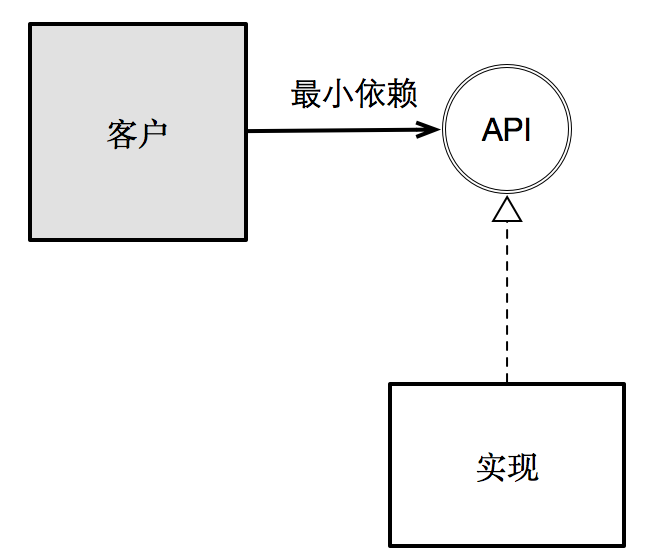
\includegraphics[width=0.5\textwidth]{isp.png}
  \end{figure}
\end{frame}

\subsection{向稳定的方向依赖}

\begin{frame}[fragile]{向稳定的方向依赖}
  \begin{enumerate}
    \item \alert{依赖于抽象,不要依赖于实现}
    \item \alert{倒置依赖:高层不依赖与底层,两者都依赖于抽象}
    \item \alert{按照接口编程}
  \end{enumerate}
\end{frame}

\begin{frame}[fragile]{向稳定的方向依赖: LSP}
  \begin{figure}
    \centering
    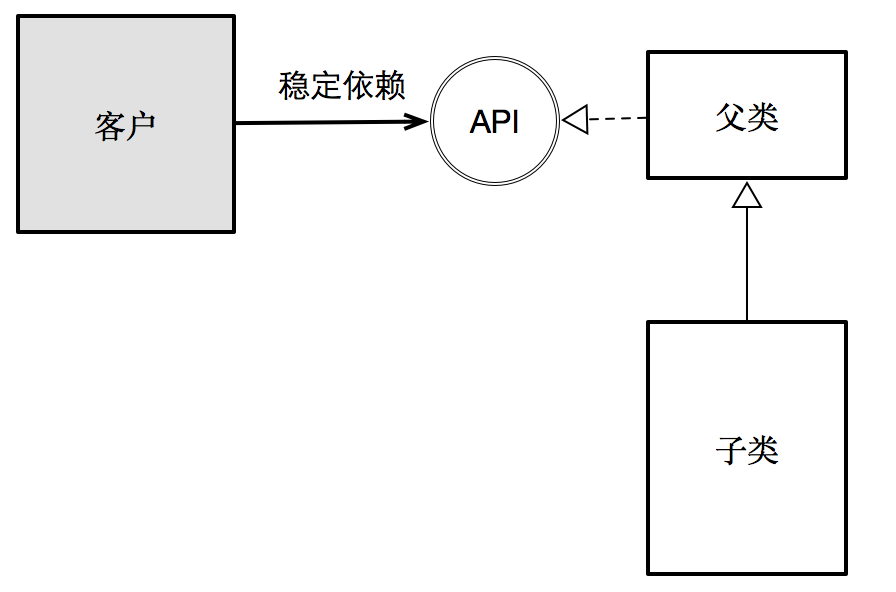
\includegraphics[width=0.6\textwidth]{lsp.png}
  \end{figure}
\end{frame}

\begin{frame}[fragile]{向稳定的方向依赖: DIP}
  \begin{figure}
    \centering
    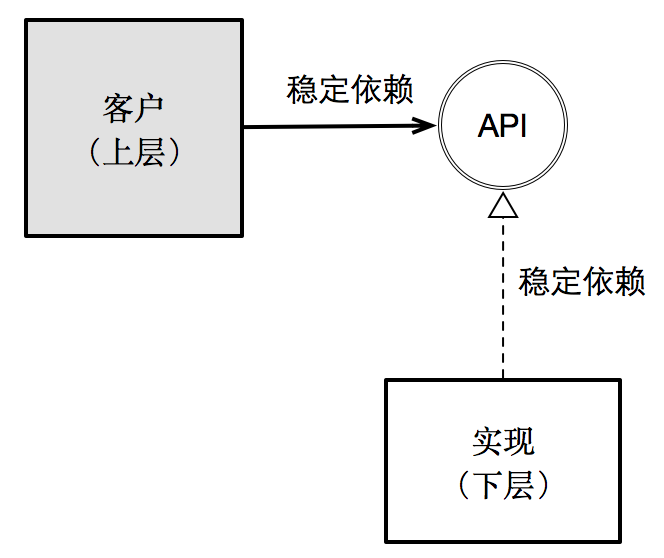
\includegraphics[width=0.5\textwidth]{dip.png}
  \end{figure}
\end{frame}
